\begin{frame}
\frametitle{1 fokú csúcsok}

\begin{columns}
\begin{column}{0.5\textwidth}
\begin{footnotesize}
\begin{itemize}
\item
\only<-2>{Csúcsok száma: $n\leq{}2k^2$}
\only<3->{Csúcsok száma: $n$ $\textcolor{red}{\leq{}k^2}$}
(pl. $1000$)
\item Élek száma: $e\leq{}k^2$
\item Kizárható vendégek száma: $k$ (pl. $10$)
\item \only<1>{Csúcsok fokszáma: $1\leq{}d(v)\leq{}k$}\only<2->{Csúcsok fokszáma: $\textcolor{red}{2\leq{}}d(v)\leq{}k$}
\end{itemize}
\emptyline
Mit tehetünk a következő csúcsokkal?
\begin{itemize}
\item A: $1$ fokszámú csúcs \uncover<2->{\textcolor{red}{$\rightarrow$ Beengedjük}}
\item B: A szomszédja \uncover<2->{\textcolor{red}{$\rightarrow$ Kitiltjuk, k-t csökkentjük}}
\end{itemize}

\begin{itemize}
\uncover<4->{\item ${{k^2}\choose{k}}$, pl. ${{100}\choose{10}} \approx 1.73\cdot10^{13}$.\\
Már a laptopunk is le tudja futtatni!}
\end{itemize}
\end{footnotesize}
\end{column}

\begin{column}{0.5\textwidth}
\begin{center}
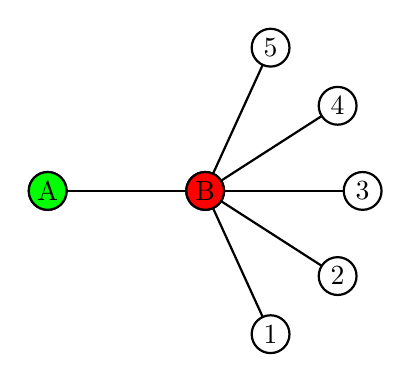
\begin{tikzpicture}[scale=2]
\coordinate (N1) at (1.41542,0.09037);
\coordinate (N2) at (1.84125,0.45936);
\coordinate (N3)  at (2.00000,1.00000);
\coordinate (N4)  at (1.84125,1.54064);
\coordinate (N5)  at (1.41542,1.90963);
\coordinate (A)   at (0.00000,1.00000);
\coordinate (B)   at (1.00000,1.00000);
\draw[thick] (B) -- (N1);
\draw[thick] (B) -- (N2);
\draw[thick] (B) -- (N3);
\draw[thick] (B) -- (N4);
\draw[thick] (B) -- (N5);
\draw[thick] (A) -- (B);
\draw[thick, fill=white] (N1)  circle (0.12) node{1};
\draw[thick, fill=white] (N2)  circle (0.12) node{2};
\draw[thick, fill=white] (N3)  circle (0.12) node{3};
\draw[thick, fill=white] (N4)  circle (0.12) node{4};
\draw[thick, fill=white] (N5)  circle (0.12) node{5};
\uncover<1>{\draw[thick, fill=white] (A)   circle (0.12) node {A};}
\uncover<2->{\draw[thick, fill=green] (A)   circle (0.12) node {A};}
\uncover<1>{\draw[thick, fill=white] (B)   circle (0.12) node {B};}
\uncover<2->{\draw[thick, fill=red]   (B)   circle (0.12) node {B};}
\end{tikzpicture}
\end{center}
\end{column}
\end{columns}

\end{frame}

